\section{Слой бизнес-логики}
	Слой бизнес логики был реализован с помощью использования шаблона "Модель предметной области". Все классы, реализующий слой бизнес-логики разделены на два пакета:
	\begin{itemize}
		\item \texttt{entity} --- в данном пакете описаны все сущности, определенные в системе;
		\item \texttt{logic} --- в данном пакете описаны все классы, реализующие бизнес-логику системы.
	\end{itemize}
	
	\subsection{Пакет \texttt{entity}}
	В данном пакете описаны все сущности, над которыми оперирует бизнес-логика. Диаграмма классов пакета \texttt{entity} приведена на рисунке~\ref{fig:entityDiagram}.
	\begin{figure}[h]
		\center{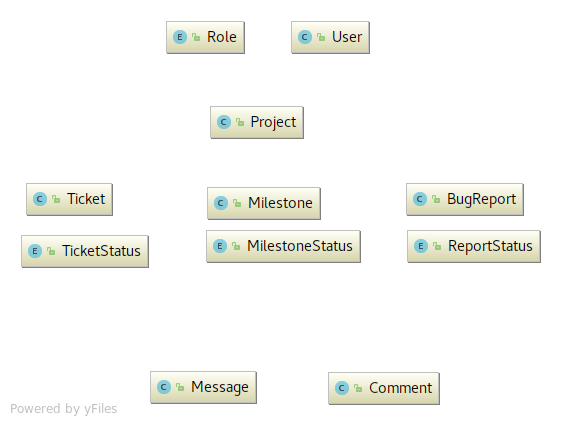
\includegraphics[width=\linewidth]{entityDiagram}}
		\caption{Диаграмма классов пакета \texttt{entity}}
		\label{fig:entityDiagram}
	\end{figure}
	
	Все классы данного пакета являются сущностными, т.е. они лишь хранят необходимые данные и имеют методы для получения/записи этих данных. Рассмотрим классы данного пакета более подробно.
	\begin{itemize}
		\item \texttt{User} --- класс, описывающий пользователя. Данный класс хранит: уникальный идентификатор пользователя; уникальный логин пользователя; имя; пароль и список уведомлений, полученных данным пользователем.
		
		\item \texttt{Project} --- класс, описывающий проект. Данный класс хранит: уникальный идентификатор пользователя; уникальное имя проекта; указатель на менеджера проекта; указатель на тимлидера проекта~(если он определен); список разработчиков; список тестировщиков; список майлстоунов; список сообщений об ошибках.
		
		\item \texttt{BugReport} --- класс, описывающий сообщение об ошибке. Данный класс хранит: уникальный идентификатор отчета; указатель на проект~(к которому он привязан); указатель на автора отчета об ошибке; указатель на разработчика, который исправляет данную ошибку~(если он определен); описание ошибки; список комментариев к данной ошибке.
		
		\item \texttt{Milestone} --- класс, описывающий майлстоун. Класс хранит: уникальный идентификатор; проект, к которому привязан; текущий статус; предполагаемое время начало майлстоуна; время, когда майлстоун действительно был начат; предполагаемое время завершения майлстоуна; время, когда майлстоун был дейтсвительно завершен; список тикетов, привязанных к данному майлстоуну.
		
		\item \texttt{Ticket} --- класс, описывающий тикет. Класс хранит: уникальный идентификатор; указатель на майлстоун, к которому привязан; указатель на создателя тикета; текущий статус; список разработчиков, назначенных на выполнение тикета; дату создания тикета; описание задания; список комментариев к данному тикету.
		
		\item \texttt{Comment} --- класс, описывающий комментарий к тикету или отчету об ошибке. Класс хранит: уникальный идентификатор; дату создания комментария; указатель на пользователя, который оставил комментарий; текст комментария.
		
		\item \texttt{Message} --- класс, описывающий уведомления пользователя. Класс хранит: уникальный идентификатор; дату создания уведомления; указатель на пользователя, которому отправлено уведомление; текст уведомления.
	\end{itemize}
	
	\subsection{Пакет \texttt{logic}}
	В данном пакете описана вся бизнес-логика системы. Диаграмма классов пакета \texttt{logic} приведена на рисунке~\ref{fig:logicDiagram}.
	\begin{figure}[h]
		\center{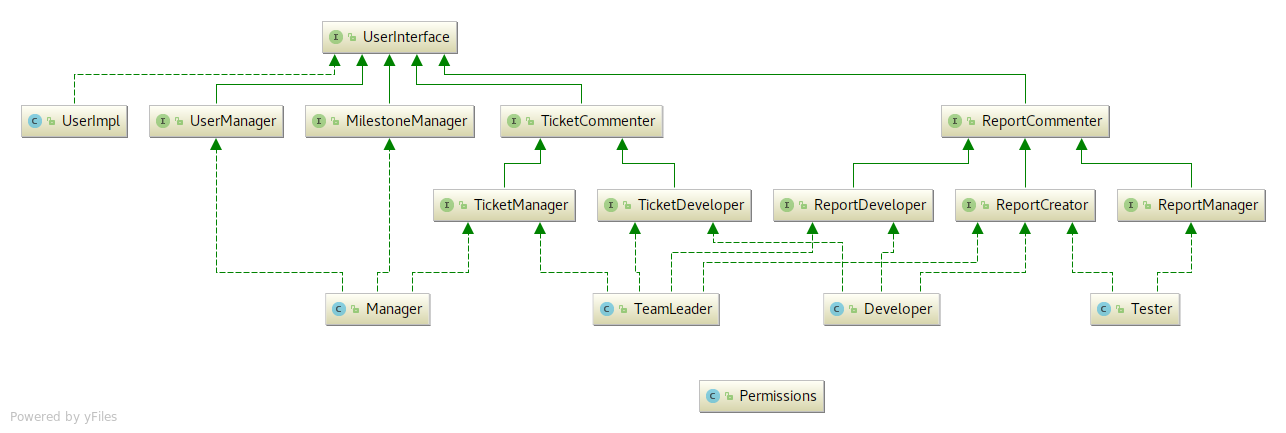
\includegraphics[width=\linewidth]{logicDiagram}}
		\caption{Диаграмма классов пакета \texttt{logic}}
		\label{fig:logicDiagram}
	\end{figure}
	
	Бизнес логика в данном пакете описывается на уровне интерфейсов, а классы соответствуют ролям и реализуют соответствующие интерфейсы. Рассмотрим их более подробно.
	
	\begin{itemize}
		\item \texttt{UserInterface} --- базовый интерфейс пользователя. Имеет методы:
		\begin{itemize}
			\item \texttt{getUser()} --- получить пользователя, к которому привязан текущий объект.
			\item \texttt{addMessage(String message)} --- добавить новое уведомление данному пользователю.
		\end{itemize}
		
		\item \texttt{UserImpl} --- класс, который реализует базовый интерфейс пользователя.
		
		\item \texttt{UserManager} --- интерфейс, в котором реализованы методы управления пользователями проекта. Расширяет интерфейс \texttt{UserInterface}. Методы могут выбросить два исключения: \texttt{MultipleRoleException} если какому-то пользователю пытаются присвоить две роли в проекте и \texttt{NoRightsException} если у текущего пользователя нет прав на управление пользователями проекта. Имеет методы:
		\begin{itemize}
			\item \texttt{setTeamLeader(Project project, User teamLeader)} --- добавить нового тимлидера к проекту.
			\item \texttt{addDeveloper(Project project, User developer)} --- добавить нового разработчика в проект.
			\item \texttt{addTester(Project project, User tester)} --- добавить нового тестировщика в проект.	
		\end{itemize}
		
		\item \texttt{MilestoneManager} --- интерфейс, в котором реализованы методы управления майлстоуном. Расширяет интерфейс \texttt{UserInterface}. Имеет методы:
		\begin{itemize}
			\item \texttt{createMilestone(Project project, Date start, Date end)} --- добавить новый майлстоун в проект.
			\item \texttt{activateMilestone(Milestone milestone)} --- сделать майлстоун активным.
			\item \texttt{closeMilestone(Milestone milestone)} --- закрыть майлстоун.	
		\end{itemize}
		
		Выбрасывает следующие исключения:
		\begin{itemize}
			\item \texttt{NoRightsException} --- если у текущего пользователя нет прав на управление проектами.
			\item \texttt{TwoActiveMilestonesException} --- если пытаемся сделать одновременно два майлстоуна активными.
			\item \texttt{WrongStatusException} --- если пытаемся установить майлстоуну неправильный статус.	
			\item \texttt{MilestoneTicketNotClosedException} --- если пытаемся закрыть майлстоун, у которого закрыты не все тикеты.	
		\end{itemize}
		
		\item \texttt{TicketCommenter} --- интерфейс, который реализует метод комментирования тикетов. Расширяет интерфейс \texttt{UserInterface}.
		
		\item \texttt{TicketManager} --- интерфейс, в котором реализованы методы управления тикетом. Расширяет интерфейс \texttt{TicketCommenter}. Имеет методы:
		\begin{itemize}
			\item \texttt{checkTicketManagerPermissions(Ticket ticket)} --- проверить права текущего пользователя на управление данным тикетом.
			\item \texttt{createTicket(Milestone milestone, String task)} --- создать новый тикет.
			\item \texttt{addAssignee(Ticket ticket, User developer)} --- добавить нового разработчика в тикет.	
			\item \texttt{reopenTicket(Ticket ticket)} --- переоткрыть тикет.
			\item \texttt{closeTicket(Ticket ticket)} --- закрыть тикет.
		\end{itemize}
		
		Выбрасывает следующие исключения:
		\begin{itemize}
			\item \texttt{NoRightsException} --- если у текущего пользователя нет прав на управление тикетом.
			\item \texttt{MilestoneAlreadyClosedException} --- если пытаемся создать новый тикет в майлстоуне, который уже закрыт.
		\end{itemize}
		
		\item \texttt{TicketDeveloper} --- интерфейс, в котором реализованы методы управления тикетом. Расширяет интерфейс \texttt{TicketCommenter}. Имеет методы:
		\begin{itemize}
			\item \texttt{checkTicketDeveloperPermissions(Ticket ticket)} --- проверить права текущего пользователя на разработку данного тикета.
			\item \texttt{acceptTicket(Ticket ticket)} --- поставить тикету статус "принят".
			\item \texttt{setInProgress(Ticket ticket)} --- поставить тикету статус "выполняется".	
			\item \texttt{finishTicket(Ticket ticket)} --- поставить тикету статус "завершен".
		\end{itemize}
		
		Выбрасывает исключение \texttt{NoRightsException} если у текущего пользователя нет прав на разработку тикета.
		
		\item \texttt{ReportCommenter} --- интерфейс, который реализует метод комментирования отчетов об ошибках. Расширяет интерфейс \texttt{UserInterface}.
		
		\item \texttt{ReportCreator} --- интерфейс, в котором реализованы методы создания отчетов об ошибках. Расширяет интерфейс \texttt{ReportCommenter}. Имеет методы:
		\begin{itemize}
			\item \texttt{checkReportCreatorPermissions(BugReport report)} --- проверить права текущего пользователя на создание отчетов об ошибках.
			\item \texttt{createReport(Project project, String description)} --- создать новый отчет об ошибке.
		\end{itemize}
		
		Выбрасывает исключение \texttt{NoRightsException} если у текущего пользователя нет прав на создание отчетов об ошибках.
		
		\item \texttt{ReportDeveloper} --- интерфейс, в котором реализованы методы исправления ошибок проекта. Расширяет интерфейс \texttt{ReportCommenter}. Имеет методы:
		\begin{itemize}
			\item \texttt{checkReportDeveloperPermissions(BugReport report)} --- проверить права текущего пользователя на исправление ошибок проекта.
			\item \texttt{acceptReport(BugReport report)} --- принять отчет об ошибке на исправление.
			\item \texttt{fixReport(BugReport report)} --- установить статус "исправлен" отчету об ошибке.
		\end{itemize}
		
		Выбрасывает следующие исключения:
		\begin{itemize}
			\item \texttt{NoRightsException} --- если у текущего пользователя нет прав на исправление ошибок проекта.
			\item \texttt{AlreadyAcceptedException} --- если пытаемся принять на исправление отчет, который уже принят другим пользователем.
		\end{itemize}
		
		\item \texttt{ReportManager} --- интерфейс, в котором реализованы методы управления отчетами об ошибках. Расширяет интерфейс \texttt{ReportCommenter}. Имеет методы:
		\begin{itemize}
			\item \texttt{checkReportManagerPermissions(BugReport report)} --- проверить права текущего пользователя на  управление отчетами об ошибках.
			\item \texttt{reopenReport(BugReport report)} --- переоткрыть отчет об ошибке, если она не была исправлена.
			\item \texttt{closeReport(BugReport report)} --- закрыть отчет об ошибке.
		\end{itemize}
		
		Выбрасывает исключение \texttt{NoRightsException} если у текущего пользователя нет прав на управление отчетами об ошибках.
		
		\item \texttt{Manager} --- класс, который описывает роль менеджера проекта. Реализует интерфейсы \texttt{MilestoneManager}, \texttt{UserManager} и \texttt{TicketManager}.
		
		\item \texttt{TeamLeader} --- класс, который описывает роль тимлидера проекта. Реализует интерфейсы \texttt{ReportCreator}, \texttt{ReportDeveloper}, \texttt{TicketManager}, \texttt{TicketDeveloper}.
		
		\item \texttt{TeamLeader} --- класс, который описывает роль разработчика проекта. Реализует интерфейсы \texttt{ReportCreator}, \texttt{ReportDeveloper}, \texttt{TicketDeveloper}.
		
		\item \texttt{TeamLeader} --- класс, который описывает роль тестировщика проекта. Реализует интерфейсы \texttt{ReportCreator}, \texttt{ReportManager}.
		
		\item \texttt{Permissions} --- класс, который хранит права пользователя для какого-то проекта в виде битовой маски.
	\end{itemize}